\documentclass[a4paper,11pt,twoside,openright]{report}

\usepackage{graphicx}
%\usepackage{ngerman}
\usepackage[utf8x]{inputenc}
\usepackage{fancyvrb}
\usepackage{courier}
\usepackage{helvet}
\usepackage{tikz}
\usepackage{xcolor}
\usepackage{pdfpages}
\usepackage[strict]{changepage}
\usepackage{verbatim}

\pdfoptionpdfminorversion=6

% \definecolor{se_dark_blue}{RGB}{0,103,166} % powerpoint
\definecolor{se_dark_blue}{RGB}{0,96,178} % website
% \definecolor{se_light_blue}{RGB}{119,158,201} % powerpoint
\definecolor{se_light_blue}{RGB}{129,160,225} % website


%% setup listings
\usepackage{listings}
\lstset{
    numbers=left,
    numberstyle=\tiny,
    numbersep=5pt,
    xleftmargin=11pt,
    xrightmargin=4pt,
    frame=single,
    aboveskip=0pt,
    belowskip=-6pt,
    sensitive=true,
    float=!t,
    breaklines=false,
    captionpos=b,
    tabsize=2,
    showstringspaces=false,
    basicstyle=\small\ttfamily,
    morecomment=[l]{//},
    morecomment=[s][\itshape]{/**}{*/}
}

%% defines the listings laguage named 'MontiArc' derived from the language 'Java' 
%% adding the below listed keywords. See 
%% ftp://ftp.tex.ac.uk/tex-archive/macros/latex/contrib/listings/listings.pdf
%% for listings documentation
\lstdefinelanguage{MontiArc}[]{Java}{
  morekeywords={component, port, in, out, inv, package, import, connect, autoconnect}
}

% Seite einrichten
\setlength{\voffset}{-1in}
\setlength{\hoffset}{-1in}

\setlength{\topmargin}{2.5cm}		   
\setlength{\headheight}{0cm}		   
\setlength{\headsep}{0cm}		   
\setlength{\oddsidemargin}{3,3cm}  % innen ein wenig mehr Rand für die Klebebindung
\setlength{\evensidemargin}{2,7cm} % dafür außen ein wenig weniger
\setlength{\textwidth}{15cm}		   
\setlength{\textheight}{23,5cm}		   
\setlength{\parindent}{0cm}

\newcommand{\emptyLine}{{\LARGE ~\\}}

\setcounter{tocdepth}{2}  %table of contents depth

\begin{document}

% Einrücken von Absätzen verhindern und 1.5 Zeilen Absatzabstand
\setlength{\parindent}{0pt}
\setlength{\parskip}{1.5ex plus0.5ex minus0.5ex}

%% Dieses Teildokument beschreibt die Titelseite.
%

% Seitenzähler auf 1, Römische Ziffern.
\setcounter{page}{1}
\pagenumbering{roman}

\thispagestyle{headings}

%\changepage{<text height>}{<text width>}{<even-side margin>}{<odd-side margin>}{<column sep.>}{<topmargin>}{<headheight>}{<headsep>}{<footskip>}
\changepage{5,1cm}{2.4cm}{}{-0.7cm}{}{-2,3cm}{}{}{}

% Eigentliche Titelseite.
\begin{titlepage}
	
\begin{figure}\raggedleft
\includegraphics[height=3.0cm]{src/pic/logo.jpg}\end{figure}
  
\begin{tikzpicture}[overlay]

% horizontal lines
\draw[color=se_dark_blue, thick] (-1.6, 0.9) -- (17.4, 0.9);
\draw[color=se_light_blue, thick] (-1.4, 0.7) -- (17.4, 0.7);

% vertical lines
\draw[color=se_dark_blue, thick] (-1, 0.9) -- (-1, -24.5);
\draw[color=se_light_blue, thick] (-0.8, 0.7) -- (-0.8, -24.5);

\end{tikzpicture}

\vspace*{-1.5em}

\begin{flushleft}
  {\fontfamily{phv}  
  	{\LARGE
      Rheinisch Westfälische Technische Hochschule Aachen \\
      Lehrstuhl für Software Engineering \\}
    \vspace{3em}
  
    {\LARGE \textbf{Erste Titel-Zeile}\\} 
    {\LARGE \textbf{Zweite Titel-Zeile}\\} 
    {\LARGE \textbf{Dritte Titel-Zeile}\\} % Oder \emptyLine falls nicht Titel kürzer
    {\LARGE \textbf{Vierte Titel-Zeile}\\} % Oder \emptyLine falls nicht Titel kürzer
    \vspace{3em}
		
    {\Large \textbf{Diplomarbeit/Masterarbeit/Studienarbeit}\\}
		\vspace{3em} 
		
		{\large von\\} % presented by
    
    {\LARGE \textbf{Name, Vorname}\\}
    \vspace{3em} 
		    
    {\Large \textbf{1. Prüfer: Prof.\ Dr.\ B.\ Rumpe}\\}
    \vspace{1em} 
    {\Large \textbf{2. Prüfer: }\\}
    \vspace{1em} 
    {\Large \textbf{Betreuer: }\\}
    \vspace{7em} 

    {\large Diese Arbeit wurde vorgelegt am Lehrstuhl für Software Engineering \\}
    \vspace{1em}
    % The present work was submitted to the chair of software engineering
		{\large	Aachen, den \today\\}
  }
\end{flushleft}

\end{titlepage}

\changepage{-5,1cm}{-2.4cm}{}{0.7cm}{}{2,3cm}{}{}{}





%Dieses Teildokument beschreibt die Titelseite.
%

% Seitenzähler auf 1, Römische Ziffern.
\setcounter{page}{1}
\pagenumbering{roman}

\thispagestyle{headings}

%\changepage{<text height>}{<text width>}{<even-side margin>}{<odd-side margin>}{<column sep.>}{<topmargin>}{<headheight>}{<headsep>}{<footskip>}
\changepage{5,1cm}{2.4cm}{}{-0.7cm}{}{-2,3cm}{}{}{}

% Eigentliche Titelseite.
\begin{titlepage}
	
\begin{figure}\raggedleft
\includegraphics[height=3.0cm]{src/pic/logo.jpg}\end{figure}
  
\begin{tikzpicture}[overlay]

% horizontal lines
\draw[color=se_dark_blue, thick] (-1.6, 0.9) -- (17.4, 0.9);
\draw[color=se_light_blue, thick] (-1.4, 0.7) -- (17.4, 0.7);

% vertical lines
\draw[color=se_dark_blue, thick] (-1, 0.9) -- (-1, -24.5);
\draw[color=se_light_blue, thick] (-0.8, 0.7) -- (-0.8, -24.5);

\end{tikzpicture}

\vspace*{-1.5em}

\begin{flushleft}
  {\fontfamily{phv}  
  	{\LARGE
      RWTH Aachen University \\
      Software Engineering Group \\}
    \vspace{3em}
  
    {\LARGE \textbf{Spike\ Train\ Analysis\ in\ Mechanically}\\} 
    {\LARGE \textbf{Stimulated\ Rat\ Neural\ Fibers:}\\} 
    {\LARGE \textbf{Use\ Case\ for\ Design\ of\ OpenMNGlab\ Software}\\} % Replace with \emptyLine if title is shorter
    %{\LARGE \textbf{Forth line of title}\\} % Replace with \emptyLine if title is shorter
    \vspace{3em}
		
    {\Large \textbf{Bachelor Thesis}\\}
		\vspace{3em} 
		
		{\large presented by\\} 
    
    {\LARGE \textbf{Tartsch, Alexander Manuel}\\}
    \vspace{3em} 
		    
    {\Large \textbf{1st Examiner: Prof.\ Dr.\ rer.\ nat.\ A.\ Morrison}\\}
    \vspace{1em} 
    {\Large \textbf{2nd Examiner: apl.\ Prof.\ Dr.\ med.\ B.\ Namer}\\}
    \vspace{1em} 
    {\Large \textbf{Advisor: Dr.\ rer.\ medic.\ E.\ Kutafina}\\}
    \vspace{1em} 
    {\Large \textbf{Advisor: M.\ Sc.\ A.\ Pérez\ Garriga}\\}
    \vspace{7em} 

    {\large The present work was submitted to the Chair of Software Engineering \\}
    \vspace{1em}
    % The present work was submitted to the chair of software engineering
		{\large	Aachen, \today\\}
  }
\end{flushleft}

\end{titlepage}

\changepage{-5,1cm}{-2.4cm}{}{0.7cm}{}{2,3cm}{}{}{}




 % English cover

\clearpage

% Erklaerung

%\includepdf[pages={1},offset=-1in -1in]{Formular_Eidesstattliche_Versicherung_neu.pdf}
%\includepdf[pages={1},offset=-1in -1in]{Statutory_Declaration_in_Lieu_of_an_Oath.pdf} % English 

%\clearpage

\vspace*{2cm}
% Abstract
{\bf\Large Kurzfassung} \\ [1em] 
Eine kurze Zusammenfassung der Arbeit.

\vspace{10ex}
{\bf\Large Abstract} \\ [1em]
A short abstract of this thesis.

\cleardoublepage


\tableofcontents

\clearpage

% Ab erstem Kapitel Seiten arabisch zählen
\setcounter{page}{1}
\pagenumbering{arabic}

\chapter{Introduction}
\begin{comment}
In this chapter I will give an introduction to the topic. I will give background information about neuropathic pain and the big picture goal of research in this field. \\
-quickly explain how the transmission of pain functions inside our bodies\\
-what is my bachelor thesis based on (paper from Roberto)\\
-contextualize thesis topic within the big picture \\
-talk quickly about openMNGlab and goal of adding analysis functionality and discuss software engineering goals for the framework\\

nociception/pain\\
neuropathic pain -> constant firing\\
measuring data -> microneurography\\
analyzing data -> openMNGlab\\
results -> ideas for problemsolving

C fibers
when these fibers fire all the time this is called neuropathic pain
\end{comment}
\section{Pain and Nociception}
%This section describes the general concept of nociception and pain.\\
%Nociception is what happens when we experience noxious stimuli. Pain is what our brain interprets these stimuli as.
An important field of study in the medical sciences is the study of pain. The IASP defines pain as "an unpleasant sensory and emotional experience associated with, or resembling that associated with, actual or potential tissue damage". The IASP is the international association for the study of pain. It is the leading global organization supporting the study and practice of pain and pain relief~\cite{iasp_2022}. \\
It is important to distinguish pain from the neurally coded response to potentially harmful stimuli, which is called nociception. The definition of pain includes the internal experience, as well as the concrete stimulus response.\\
As a result of a lesion or disease of the somatosensory nervous system people can also experience chronic neuropathic pain. Studies suggest, that around 6-10\% of people in the general population suffer from neuropathic pain~\cite{bouhassira_prevalence_2008}~\cite{van_hecke_neuropathic_2014}. Treatments for this are limited and often have side effects, which makes this disease difficult to deal with~\cite{brooks2017treatments}.\\
In order to study this further we need to understand the basic principles of how physical stimuli are transmitted and lead to potential pain in the brain.

\section{Neural Signalling}
After a stimulus is received by a corresponding receptor, the information needs to be passed to the brain.
The way that signals are transmitted from sensory input to the brain is via electrical signals inside of nerve fibers. Because signals have to travel aver a longer distance in the human body, the information is coded not in a continuous signal but through discrete events called action potentials or spikes~\cite{rieke1999spikes}~\cite{spikeGeneral}.\\
Spikes are an all or nothing event, which means that the concrete spike shape does not have an effect on the encoded message. It has been shown that information is temporally encoded via patterns and firing rates of spikes.\\
Trying to figure out how exactly information gets encoded has been a long standing research question.\\
In order to understand aspects of the neural code we want to analyze spiking patterns in C-fibers evoked by a mechanical stimulus. This might give us small hints about the encoding of information within the neural network. \\
One method to record such data is called microneurography (MNG). It is an electrophysiological technique that can measure peripheral nerve activity in awake human subjects~\cite{namer2009translational}. A needle electrode is inserted into a peripheral nerve and records its responses to stimuli. With this we only look at spikes from a single neuron, however, in reality signals are passed and processed by large quantities of neuronal clusters and what we are looking at is only a small part of encoding information~\cite{spikeGeneral}.\\
In this thesis we take a look at MNG data from Roberto de Col and try to replicate some of his analysis~\cite{roberto} using the software framework openMNGlab~\cite{schlebusch_openmnglab_2021}. While doing this take a closer look at how this particular use case is handled by the software and where it can be improved.

\section{Results}
I tested importing experimental files into openMNGlab and added some analysis code. In the end I managed to import 22 files, although with some difficulties and patchwork code. These problems lead me to propose some improvements for the software. Apart from the import of the 22 files I also added some analysis code and included the results of the analysis of one of the files in detail in this thesis.\\
I replicated some of the analysis methods used in~\cite{roberto} and concluded with the same results. We found that increased spiking activity of a nerve fiber, here evoked through electrical stimulation, leads to decreased response to a mechanical stimulus. In addition I also tried some other quantification approaches for the spike train data and added visualizations for the sample analysis.

% Die Logos sind veraltet und duerfen zurzeit nicht verwendet werden!
% Auf Seite \pageref{Logo} in Abbildung \ref{Logo} befindet sich das SE Logo.
\begin{comment}
-Neuropathic pain as basis \\
-comes with many diseases \\ 

-pain as electric signals \\
-goal to understand the firing patterns in nerve fibers \\
-microneurography as recording technique \\
-needle in vitro in patients \\
-action potentials as spikes \\
-animal data \\
-does not need fiber separation  

-OpenMNGlab \\
-currently only good for loading the data \\
-want to add analysis capabilities \\
-compute quantifiers for spike trains and recordings \\
-discuss results 
 
Software: \\
-working on jupyter notebook \\
-automate the spike analysis process \\
-integrate analysis into openMNGlab \\
-get requirements for spike analysis software 


There are many unsolved problems in the medical sciences. The one connected to this bachelor thesis is the issue of neuropathic pain.
This is a type of chronic pain that can appear at any moment without any obvious factors coming from the outside. It can stem from diseases that effect the nerves, but also from infection or injury.\\
%-TODO find number of people in Germany that suffer from neuropathic pain\\
%-TODO: Find out more details on neuropathic pain \\
Pain is transmitted as electric signals through the nerves inside our bodies. Because of this fact in order to understand different types of pain such as neuropathic pain we need to understand the transmission of electrical signals in nerve fibers.\\
Quantifying pain can be done by measuring the electrical activity of corresponding nerve fibers. By doing this we get data about the amount of electrical activity. We can also gather specifics about the way the electrical signals are being sent through the body. \\
We analyze data containing bursts of action potential activity as a potential proxy for neuropathic pain as the end goal. We do this in order to potentially detect this type of pain activity in neuropathic pain patients in the future.\\
There are multiple ways in which one can measure electrical activity in human bodies. One of these methods is called microneurography, which is the technique most relevant for the rest of this thesis.
This technique is used to record nerve activity in peripheral nerves. With this technique typically a needle gets inserted into a nerve fiber which then detects the electrical current in the fiber. Additionally, we can stimulate the nerve fiber to get certain responses. \\
Nerve fibers transmit data with the use of action potentials, short AP or spike. It has been shown in previous research that information is not transmitted by the shape or amplitude of the spikes, but the frequency and timings(reference). \\

%\section{Action potentials}
Action potentials, also called spikes, are ...\\
It has been shown that coding of information is done in the pattern of spikes. It does not matter how exactly a spike looks, spikes are treated as the same objects. 


Another aspect of this thesis is the use of a software framework for microneurography analysis. It is called OpenMNGlab and is being developed at the chair of medical informatics at the Uniklinik Aachen~\cite{schlebusch_openmnglab_2021}. Currently this framework has the capabilities to import data from different data acquisition tools, but is lacking more in depth analysis functionality. I am working on quantifying experimental data and with the help of OpenMNGlab and developing analysis functionalities, that could be integrated into OpenMNGlab in the future.

\end{comment}




\cleardoublepage


\chapter{Background}

-Available spike analysis frameworks \\
-fieldtrip \\\
-elephant \\
-Why they are not sufficient \\
-problem with the relays? maybe windows updates 

 

-openMNGlab as a solution \\
-acquisition frameworks we need to handle \\
-Current status of openMNGlab, including Neo \\
-go into detail on different data acquisition softwares \\
-Dapsys, OpenEphys, Spike2 \\
-why does dapsys not work in the future \\

  

When deciding with which software to analyze the data there were multiple possibilities. 

There are the existing FieldTrip and Elephant tools, as well as the Software framework openMNGlab,  that all offer different analysis opportunities for electrophysiology data. 

Fieldtrip (fieldtriptoolboX.org) is a software developed at the Radboud University, Nijmegen, the Netherlands and offers a wide variety of analysis functions. The main problem with this software is its programming language. It is a MATLAB toolkit, however it would be preferred to use a software package in python or another programming language that slots better in the already existing structure within the chair for medical informatics. In addition to that it is not only speficied for spike trains software, dealing with MEG, EEG and iEEG analysis. 

Elephant (https://elephant.readthedocs.io/en/latest/index.html) is a python module which offers some high-level analysis functions for spike trains specifically. The main problem with this software is the lack of basic functionalities. It relies more on highly specified analysis tools that are not necessarily viable in our use-case. For the use in this thesis I want to start with the basic signal from the spikes, try out different quantifiers and look at the data from a fresh perspective. 

In the end I decided on using the software framework openMNGlab. It is a python framework being developed at the chair of medical informatics RWTH. It offers some basic import and analysis functionalities that are ideal for using in this Bachelor thesis. With this framework I can start from the beginning and develop my own quantifiers. 


\section{Data acquisition software} 
There are many different data acquisition software packages for electrophysiological data. 

\subsection{Spike2}
“Spike2 is a multi-channel continuous data acquisition and analysis package”( https://ced.co.uk/products/spkovin) produced by Cambridge electronic design limited. \\
-Used for the experiments I am analysing by Roberto \\
-records data in multiple channels \\
-channel for raw signal \\
-channel for mechanical force \\
-channel for event markers \\
-channel for temperature (not used by me) \\
-channel for comments (used for marking when chemicals are applied) \\
-spikes can be separated into own channels (done by experimenters) \\
-software offers a graphical representation of the data \\
-channels are separated \\
-was used for confirmation of what the data should output in terms of basic quantifiers \\
-can export csv files from the data \\
-has direct importer in openMNGlab \\

Spike2 is a data acquisition and analysis software produced by Cambridge electronic design limited. It is a flexible tool that can be used in a variety of different ways.

TODO: go into detail\\

\begin{figure}
	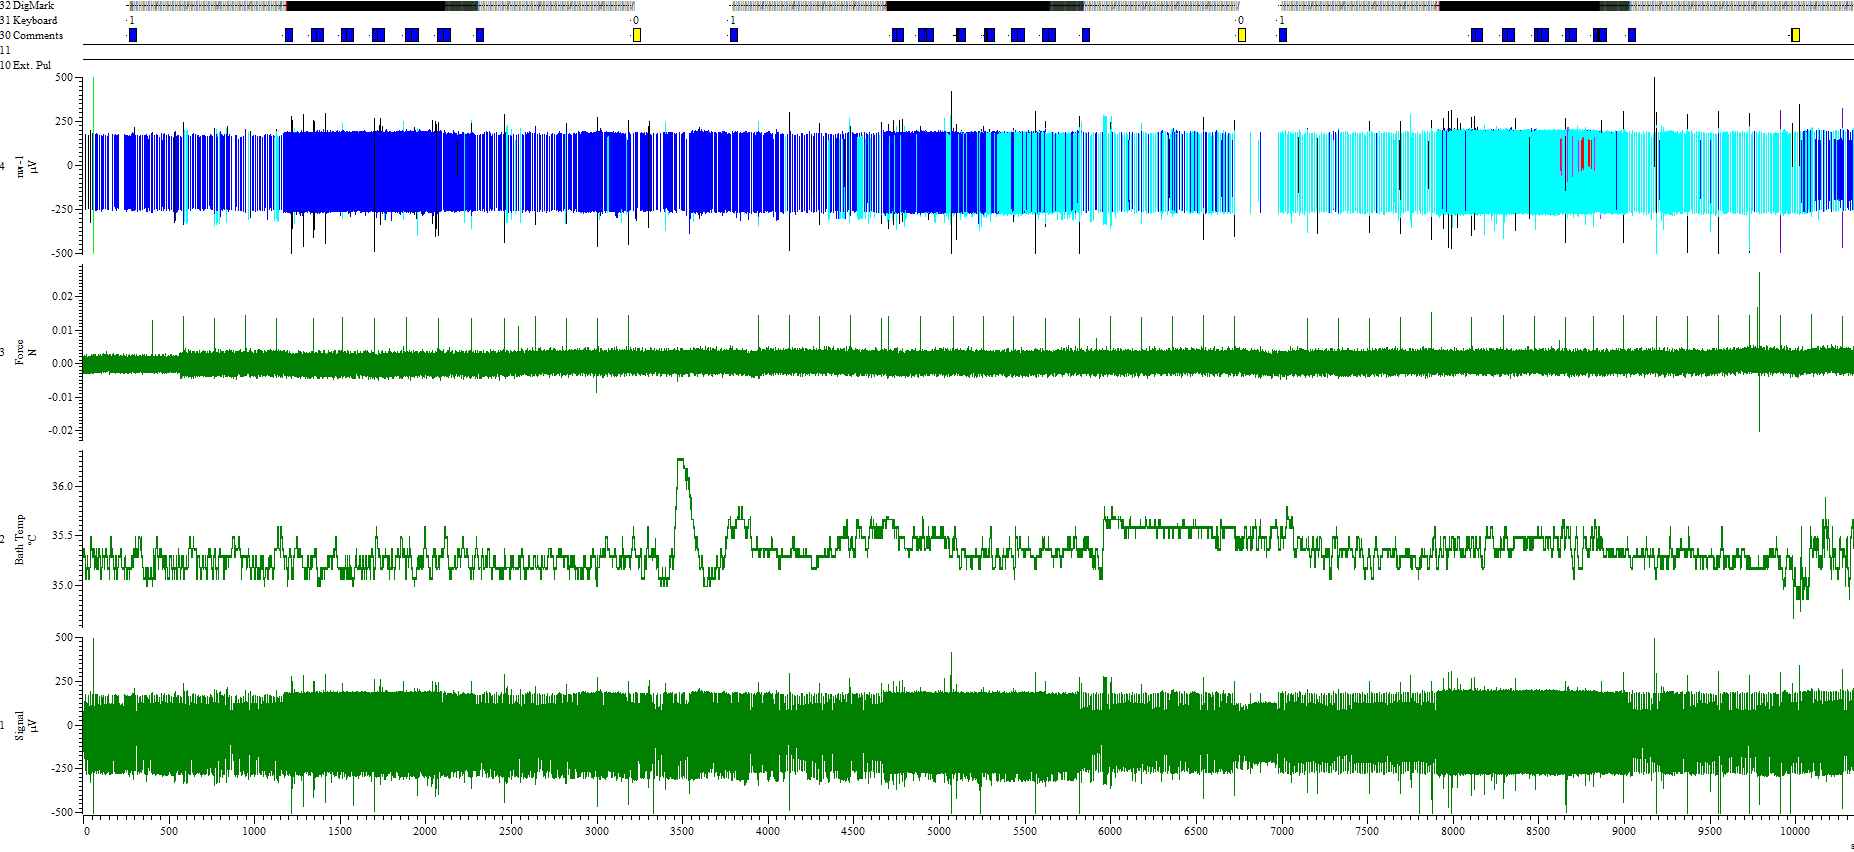
\includegraphics[width = \textwidth]{src/pic/Spike2_screenshot}
	\caption{Typical mechanically and electrically stimulated recording in Spike2}
	\label{fig:spike2}
\end{figure}

The software can record multiple channels simultaneously. An example screenshot from a recording can be seen in Figure~\ref{fig:spike2}. This depicts a typical recording used for analysis in this bachelor thesis. The recording contains data from nerve fibers of rat cranial dura mater. The nerve fibers were stimulated using a mechanoelectrostimulator applying electaical and mechanical stimulation. 

\begin{figure}
	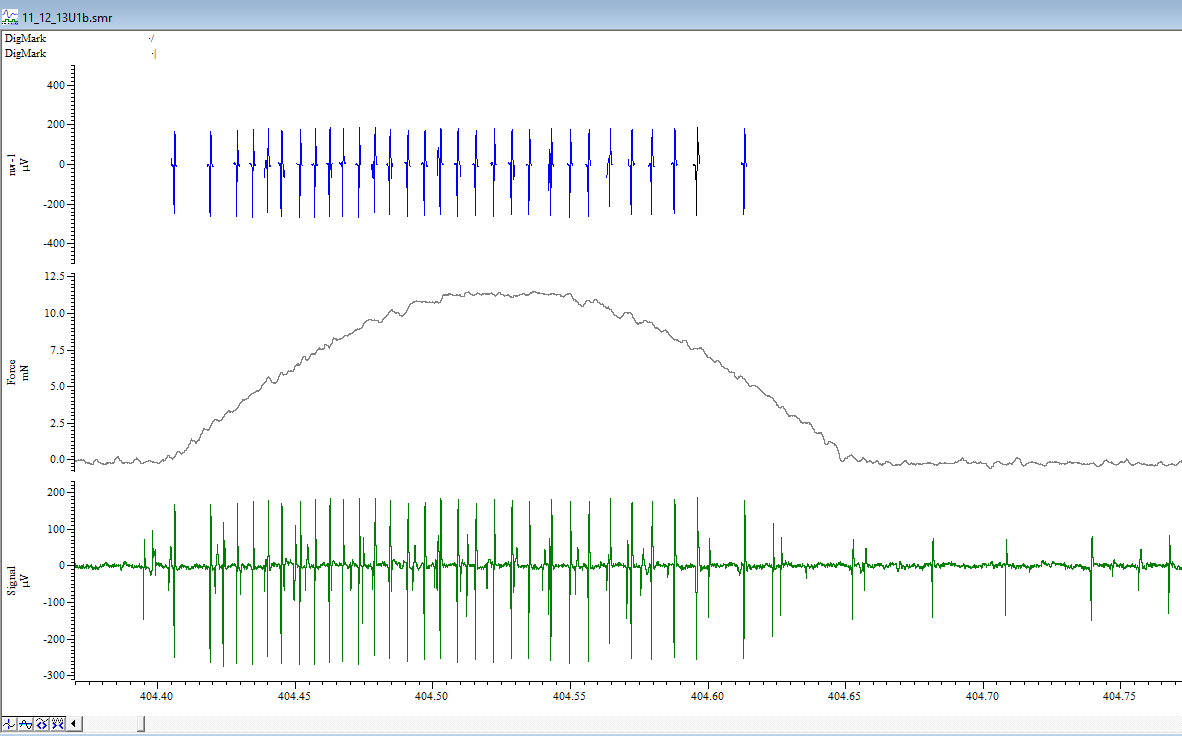
\includegraphics[width = \textwidth]{src/pic/Spike2_spike_train}
	\caption{A single spike train in spike2}
	\label{fig:spike_train}
\end{figure}

First of all it contains a channel for the recorded raw signal at the bottom. The next channel contains the temperature during the recording. In this example it fluctuates between 35°C and 36.5°C. In channel 3 we can observe the mechanical force that was applied to the nerve fibers. In Figure~\ref{fig:spike2} there are spikes in mechanical force whenever a mechanical stimulation occurs to evoke a spike train. For this experiment we want to collect the data of single nerve fibers. It is diffucult, to record just a single nerve fiber in vitro, however. This is why in this experiment spike templates are applied to the raw signal to filter out specific fibers. These filtered fibers are then displayed in channel 4, where only the action potentials of selected shapes are collected.\\
The topmost channel in Figure~\ref{fig:spike2} contains markers for the electrical and mechanical stimuli. Additionally there is a channel containing comments regarding the experiment. Comments can represent the experimental protocol and are filled in by the experimenters. In this example there are comments denoting a change electrical stimulation frequency. In other experiments for example, these could also denote the application of certain chemicals towards the recorded subject.

A more detailed view of a single spike train can be seen in Figure~\ref{fig:spike_train}. Here the difference in electrical and mechanical event markers in the topmost chanel can be seen. Mechanical markers are represented by a slash, while electrical markers are represented by a vertical line. Another thing that can be seen here is the channel containing only the spikes. This channel is ideal for the extraction of the spikes for later analysis as there is no noise in the channel anymore and the spikes can also be interpreted as simple events with a timestamp.

\subsection{Dapsys}
“DAPSYS is a combined hardware and software system designed for real-time acquisition and display of data and synchronous control of stimulators.” (http://www.dapsys.net/) \\
-Used by Barbara for her experiments \\
-used for mng-experiments with human patients \\
-also has a graphical representation of the data \\
-has importer in openMNGlab \\
-needs to export specific templates for the importer to work \\
-Dapsys has problem in the future \\
-it gets harder to set up experimental protocols \\
-maybe it has something to do with newer windows updates \\
-that means this will probably not be used much in the future \\



\subsection{OpenEphys}
OpenEphys \\
-open-source electrophysiology \\
-based in Cambridge, Massachusetts \\
-Used in experiments in Bristol cooperation \\

 
\cleardoublepage


\chapter{Methods}
%not sure if use-cases should not go into a different chapter\\
%this chapter would then focus on just the process of developing my analysis pipeline and finish with a detailed description of it.
%\section{Chapter content}
In this chapter I will describe the methods I used for creating the software and spike analysis results in this thesis\\
-Describe the different data structures (Neo, old openMNGlab version)\\
-Detail the development process, issues during development and how they were resolved\\
-Describe the finished analysis pipeline with the help of a simplified graph\\
-present use cases (3 students analysing different data, experimental scientist)\\

Spike Analysis:\\
-Data\\
-definition of spike trains\\
-quantifiers\\


\begin{comment}
TODO:\\
-Add what I did: somewhat detailed description of my process in developing the notebook\\
-start from the notebook which was started by Radomir for custom structure (before openMNGlab)\\
-adding of importers from old openMNGlab version (code from Fabian)\\
-adding of neo importers after integration into openMNGlab\\

-Explain the details of the different structures in python (recording from old version, neo recording/block/segment, csv files)\\
-add diagram of big picture structure of openMNGlab in greater spike data analysis pipeline\\
\end{comment}
\section{Software}

\subsection{Data structure}
In this section I will present the details of the different data structures that I will use in the course of my analysis pipeline.

\subsubsection{Neo structure}
Neo models electrophysiological data in a hierarchical structure, which is depicted in Figure~\ref{fig:neostructure}. On the lowermost level we start with data objects. An $AnalogSignal$ is regularly sampled data and can contain multiple channels. An $IrregularlySampledSignal$ is similar, but does not feature a regular sampling interval, as the name suggests. A $SpikeTrain$ object contains time point data with the information when action potentials occur. These $SpikeTrain$ objects are, however, slightly different from our understanding of spike trains in this thesis. We understand a spike train as the spikes that occur resulting from one stimulus and is quite limited duration wise. The $SpikeTrain$ object in the Neo structure is a collection of all spikes during one recording and all spike trains as we see them would be contained in one such $SpikeTrain$ object.\\
$Events$ in Neo point to distinct points in time and can be used to mark stimulation events for experiments with animals for example. $Epochs$ function similar to events, but cover a duration instead of just points in time.\\
On the next layer up there are objects for grouping all of these lower level objects. The first of these objects is a $Segment$. This groups data that was simultaneously recorded. Then there are so called $Groups$ which can group data in any arbitrary way and is not restricted to the data being  in the same Segment. On the topmost layer there are $Blocks$. One $Block$ contains multiple $Segments$ and $Groups$ which in turn contain multiple data objects.\\

In case of this Bachelor thesis we are dealing with recording files from animal experiments. When importing one such file, the resulting Neo structure looks as follows: On the top level each file contains a $block$. In our case these $blocks$ contain only one $segment$, since the recordings feature a single continuous signal without interruptions.

\begin{figure}
	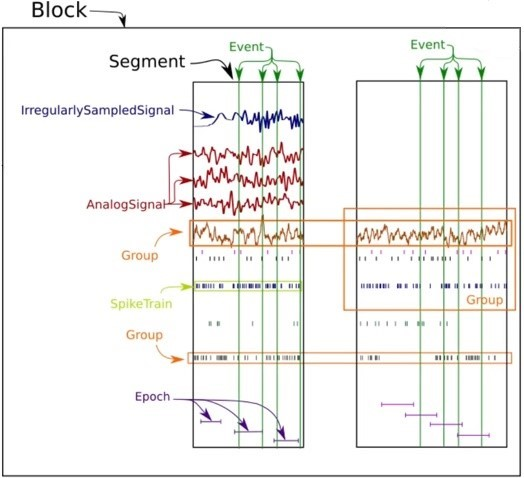
\includegraphics[width = \textwidth]{src/pic/neo_structure}
	\caption{Structure of Neos hierarchical model for electrophysiological data.}
	\label{fig:neostructure}
\end{figure}

\subsubsection{Custom Structure}
Part of my analysis is still using code from version 1 from openMNGlab where the Neo structure was not yet integrated. The importer from that version delivered the data in a custom data structure.\\
At its core the custom data structure models the data hierarchically, but the objects look a little different from the ones from Neo. At the base level there are data objects $ActionPotential$, $MechanicalStimulus$, $ElectricalStimulus$ containing information corresponding to their respective names. These objects are all part of an overlying object type called $signal\_artifact$.\\
On the top level we get an object called $recording$ when importing data with this method. one such $recording$ then contains the lists $el\_stimuli$, $mech\_stimuli$, $actpots$ which are lists containing objects of types $ElectricalStimulus$, $MechanicalStimulus$ and $ActionPotential$ respectively. Additionally there is a $raw\_signal$ object which contains the raw signal in the form of arrays.

\subsection{Development Process}
The basis of my analysis notebook started with the work of Radomir Popovich, who also worked with spike train data for IMI. He had developed a jupyter notebook based on a custom import of spike train data extracted from the Spike2 software. From this he extracted the spike trains and created figures such as event plots as seen in Figure\ref{fig:eventplot}. These event plots depict the spike trains of a single recording. Each row contains the time point data of spikes for one spike train. The x axis represents the time since the last mechanical stimulus starting at 0. These figures give a good overview with one glance over the spiking activity during mechanical stimulation for recordings.
\begin{figure}
	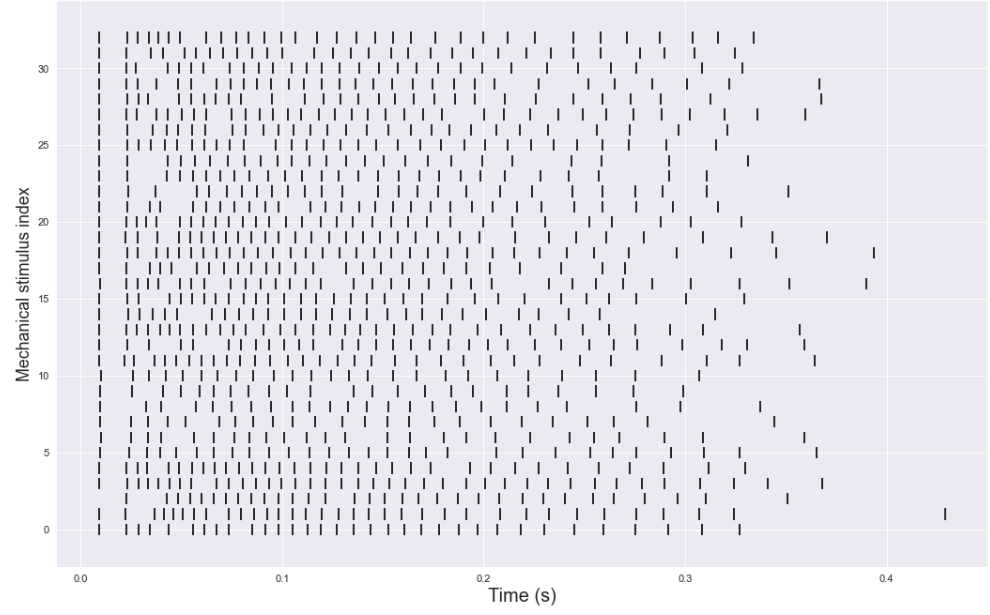
\includegraphics[width = \textwidth]{src/pic/event_plot}
	\caption{Event plot detailing spiking activity for one recording.}
	\label{fig:eventplot}
\end{figure}
Also included in this notebook was a way to filter the action potential channel so that only the relevant spikes for our spike trains remain. This was done by checking an interval of a specific duration after a mechanical stimulation event occurred for spikes and saving those in designated lists.\\
Starting of with this way of handling the data, I continued my own analysis by using the importers from version 1 of openMNGlab. Taking the extracted information of mechanically induced spike trains I started with quantifying these trains with simple numbers like duration or number of spikes per train.\\
With the further development of openMNGlab and the addition of the Neo package the importing process for the Spike2 files became a lot easier and faster. However, after a couple of attempts it became clear that the importer in its current state did not import the mechanical force channel from the experimental files. This might not be an issue when analysing other types of data, but for our use case it presents a big issue. Because the information of the mechanical force is required for the analysis I chose to combine parts of the old version of openMNGlab and parts of the new version. This way there is benefit from using the structure that Neo brings when it comes to speed and ease of use, but I am not missing information for the analysis.

%Add info about process with quantifiers



%calculation of more complex quantifiers
%graphs and diagrams

\begin{comment}
-Use-cases:\\
	\null\quad-opening data (importing)\\
	\null\quad-latency study (Alina)\\
	\null\quad-chemical data study (Jessica)\\
	\null\quad-mechanically evoked spike trains (Alexander)\\
	\null\quad-experimental researchers (Barbara)\\
-results in a list of requirements\\
-Use-cases lead to software engineering approach\\
-nessecary steps for my analysis\\
-how I implemented it
\end{comment}

\subsection{Use Cases}
To end this chapter I want to present a couple different use cases of various users of openMNGlab. I will describe the specifics of each use case and then give a few remarks on the current state of openMNGlab and the potential improvements necessary for a smoother experience for all users.

One important feature of openMNGlab that is needed in every use-case is the importing of new data. For new users it is important to be able to load sample data sets and get a feel for the framework by getting to know a few test analysis functions. For students or experimental researchers it is key to be able to load multiple files for a quick overview or even full analysis.\\
Because we are dealing with a couple of different sources when it comes to experimental data, which all need to be handled in a different way, this is where many issues can occur. When going through the use cases we will see where already we encounter some difficulties regarding the data import.



\begin{comment}
-spike2 does some automatic spike filtering
-This results in up to 20 different classes of spikes in one recording
-not all of these, however, are in fact coming from different sources
-experimental researchers have already done their own filtering with their expertise, in order to combine various different of the spike2 classified spikes into larger groups and put them in so called wavemark channels.
-previously one could export these wavemark channels to csv files and inport those into the framework
-with the direct importer from the smr files, however, this is no longer possible
-what we receive after a successful import of an smr recording file are the original spike2 classified spikes in different channels
-if one were to know which of these belong together one could easily combine those together as in spike2 with the wavemark channels
-but the information of the wavemark channels is lost during the import and so one has to manually search for the correct channels first and then combine them into groups by hand
\end{comment}

\subsubsection{Student 1}
\begin{comment}
Alina \\
Works with spike2 data \\
Electrical data and mechanical data \\
Uses old way of importing currently (csv export from spike2) \\
Needed channels from csv export: \\
DigMark for electrical and mechanical stimulus events \\
WaveMark channel for timestamps of spikes \\
Information used: \\
Electrical stimulus events + timestamps \\
Calculate Latency for spikes (timestamps) \\
Calculate Spike Count  \\
In theory this information is available with the direct import of openMNGlab right now \\
Potential problems with direct openMNGlab importer: \\
Each template for spikes in spike2 results in separate channel in Neo structure after openMNGlab import -> needs some filtering (manual right now) \\
Electrical and mechanical events share a channel (DigMark) and somehow need to be distinguished if the recording also features mechanical stimulation \\
\end{comment}

The first user is a student who does data analysis on mechanically and electrically stimulated Spike2 data. The goal is to perform latency analysis for spikes.  The raw spike2 files feature a lot of information, not all of which is always needed. In this case, all that is required to analyse the latencies of the spikes are the timestamps of the spikes itself and the timestamps of the stimulation events. For the Spike2 software this means that we need to extract the DigMark channel which contains the event information as well as the corresponding wavemark channel which contains the information on the already presorted spikes.\\
The relevant information can be imported using the importing function of openMNGlab. 
The data is then used to calculate the latency for the spikes corresponding to the latest electrical stimulus event as well as calculating the spike count.

Potential problems: The student started the analysis before the framework was working properly and therefore uses their own custom analysis notebook. However, all the information that is required is also available with the regular Spike2 importer in the current openMNGlab version.
In recordings with both electrical and mechanical stimuli, the event markers for those stimuli share the same channel in Spike2. Although they can be distinguished in Spike2 itself, the imported channel in the Neo format does not distinguish between different event types. This needs to be addressed if we want to work with recordings that feature multiple types of stimulation.
Additionally there might be some general import difficulties which I will elaborate on later in this section.
 
\subsubsection{Student 2}
\begin{comment}
Alexander \\
Works with spike2 data \\
Electrical and mechanically stimulated data \\
Uses a mixture of old and new importing currently \\
Needed channels from csv export: \\
Mechanical force channel \\
Spike channel for timestamps of spikes \\
Need channels from direct spike2 import: \\
Electrical stimulus channel \\
Information used: \\
Electrical stimulus events + timestamps \\
Mechanical stimulus events (duration, amplitude) + timestamps \\
Timestamps for spikes in spike trains \\
Potential problems with the Neo importer: \\
Each template for spikes results in separate spike channels in the Neo structure -> this means that the filtered spikes in the spike2 spike channels (e.g., nw-1…) need to be bundled together again \\
Mechanical force channel import does not work currently \\
Electrical and mechanical events share a channel (DigMark) and somehow need to be distinguished \\
After the import of the mechanical force channel, the mechanical stimuli need to be filtered as such (probably will not happen automatically by the importer) \\
\end{comment}

The second user is also a student who uses mechanically and electrically stimulated Spike2 data. Their goal is to analyse spike trains resulting from mechanical stimulation. For this they do not need all of the information contained in the raw Spike2 file. They need the event information for mechanical and electrical stimuli as well as the mechanical force information for details of the mechanical stimuli. The event information can be found in the DigMark channel of the Spike2 file and gets extracted by the Spike2 importer of openMNGlab. The mechanical force is a continual signal but appears in the form of sin shapes when the nerve is stimulated.
Just as the first user they also need the information regarding the spikes themselves, which are also imported by the framework.\\
From the gathered data the user then calculates various quantifiers for the mechanically induced spike trains such as spike count or more elaborate features. The user started this project while still using the old framework version where the channels from the Spike2 software were manually extracted to a csv file. With the updates to the framework in the meantime not all of the required information gets extracted as easily as before. This is why they use a hybrid version of the two versions of the framework where they mix and match the functions as they need them.
%it is probably clear that this user is me. Should I just say so?

Potential problems: There are similar potential problems when it comes to the event channels and regular spike channels as in the case of the first user. Additionally there are problems when it comes to the import of the mechanical force. The user started the analysis with an old version of the framework which used other importers (csv files). With this technique they could extract the mechanical force throughout the recordings. The new Neo importer still has some bugs when it comes to importing the mechanical force from the Spike2 file, which requires fixing for future users who need this information.

\subsubsection{Student 3}
\begin{comment}
Jessica \\
Works with spike2 data \\
Chemical data \\
Uses Neo importer \\
Needed channels from import: \\
Spike channels for spike timestamps \\
Information used: \\
Intervals which are relevant for the application of chemicals \\
Spikes + timestamps inside those intervals \\
Which chemicals are applied when \\
Potential problems with openMNGlab importer: \\
The chemical protocols are not automatically importable and readable; There is a channel in spike2 for comments where this information is given in theory, however, the notation of what is given and how much varies from comment to comment, and one needs a good understanding of the chemicals and potentially experimental procedure \\
Comments channel is not being imported currently, even if the chemical notes where uniform; This means one must manually reed the comment channel in the spike2 software itself and manually choose some intervals which might be promising for observing chemically induced changes in spiking activity \\
\end{comment}

The third student user of the framework works on a project to analyse Spike2 data in which certain chemicals where applied to the test subject. In contrast to the other two users, this user started with the project when the current version of openMNGlab with the integration of the Neo module already in place. This means they only made use of the new importing functions and are not stuck with certain parts from the old framework. In addition to the spiking activity, as in the previous use-cases, they also need information regarding the chemicals that are applied. They need the timings and doses of the specific chemicals. From this they need to specify a time frame where they want to monitor the spiking activity that results from the application of the chemicals.\\

Potential problems: The analysis of chemically stimulated data does bring with it its own new set of problems. There is no dedicated channel for chemical information in the Spike2 software. For this reason the chemical protocols are given in the general comment channel in Spike2. That means that the experimenter manually creates a comment every time a new chemical is applied. The issue with this is that openMNGlab does not import the comment channel. In practice the comments do not have a strict naming scheme, which would also lead to difficulties with the automatic detection of specifics regarding the chemicals. This is a problem however that does not stem from the framework, but is something that has to be addressed on the side of the experimental researchers.\\
These described problems lead to the current workflow of manually selecting a suitable time frame for interesting spiking activity some time after the chemical application; some times up to a minute (check the times again) after the chemicals where applied.

\subsubsection{Experimental researcher}
Another big group of potential users for openMNGlab are experimental researchers who produce and work with electrophysiological and microneurographical data often. They will be a big part of the user base of the framework because of the nature of their work. For them it is important that the new data sets can be easily and quickly loaded and overview statistics can be displayed.


 
\begin{comment}
Which information should available after importing data? \\
Spikes + timestamps \\
Electrical stimulation + timestamps \\
Mechanical stimulation + timestamps, duration, amplitude \\
Information about application of other stimuli (chemicals, heat…) \\
For human data: temperature?  

Spike2 \\
Spike channels + some way to group them easily (e.g., in groups from spike2 templates) \\
Electrical event channel + some way to distinguish between electrical and mechanical events \\
Mechanical force channel (maybe optional) \\
Comments channel (maybe optional) \\
Temperature (optional) (probably needed for human data) \\
\end{comment}

\begin{comment}
My steps in analysis: 

First, I used a jupyter notebook from Radomir. For this the data needed to be extracted from Spike2 directly in the Software. This export step leads to a single csv file for one recording with 5 channels: Time, Signal, Force, DigMark(stimulation events), Spikes 

Using the csv files I could extract the spike trains for each mechanical stimulation. The detection of the spike train worked as follows: The start of the spike train gets determined by the stimulation event. The length of the spike train is a previously set amount of time (in most cases 500ms). During this timeframe all spikes in the spike channel get put into a list that keeps track of the spike trains. This pretty basic detection of spike trains works well in this specific use case but has its limits when it comes to other kinds of data with other experimental protocols or just simply recordings without any protocols. Then because we do not have the exact starting points of the trains or bursting patterns this method of detection falls flat. 

This first jupyter notebook already made use of what later became openMNGlab. The import of the data was handled by the software framework. However, openMNGlab got some updates soon after which made some significant changes to how the importers work. In the new and improved framework, the importer worked on the original Spike2 files instead of the extracted csv files. This allows for more detailed representation of the data since much of the information was lost in the extraction before this update. However, with this new way of importing the data the mechanical stimulation was not able to be extracted. I still needed the information of the mechanical stimulation which was only contained in the extracted csv file. For this reason, in my analysis from here on, I used a hybrid of the old and new versions of openMNGlab until I was able to fix the new importer to also include the mechanical stimulation channel. 
\end{comment}

\section{Spike Analysis}
In this section I will describe the methods I used for analysing the spike data.

\subsection{Data}
This subsection will contain a description of the original experiment data from Roberto de Col.
\begin{comment}
This chapter describes the type of data we are working with.\\
-mechanically and electrically stimulated nerve fibers from rats\\
-describe reasoning for using animal data as opposed to human data\\
Because human nerve data is hard to obtain, we can also use animal data instead as a proxy. Animal data is usable as proxy because we can observe the nerve fibers in vitro but can better separate one single nerve fiber from others. In human data an additional step of fiber separation is necessary to differentiate between individual fibers. We can use the same experimental protocols on Animals as we would on humans. This way we can understand firing patterns of spikes and quantify them. The results can then be applied to human data. \\
In the case of this thesis, we are using the data from wistar rats. The data was recorded from 2011 to 2012 by Roberto de Col and was published in a paper (put reference). The goal of the paper was to evaluate the effects of spiking activity on the response to mechanical stimulation. 

-How much of the exact experimental details are supposed to go here as far as methodology goes, since this is a computer science thesis 

The experiments were done in vitro on peripheral nerve fibers. The fibers were mechanically and electrically stimulated via a custom made electromechanostimulator. The nerve activity was recorded using an electrode. The electrical stimulation consists of small electrical pulses that come in a controlled frequency. The mechanical force is applied in a sinusoidal shape. \\
For single recordings the mechanical force that is applied throughout stays at approximately the same level for most of the files (put for how many files this is the case), but there are exceptions where the mechanical stimulation changes in amplitude and length during one recording. 

The experimental software used for these experiments is called Spike2 and is described further in the background chapter.
\end{comment}

\subsection{Spike Train Definition}
This subsection should contain the definition we use for defining spike trains. If we need a better understanding of spike trains in the Software section this subsection might move to the background chapter.

\subsection{Quantifiers}
This subsection will contain information regarding the quantifiers that I used to analyse the spike trains.


\cleardoublepage


\chapter{Results}

\begin{comment}
In this chapter I will present the results of my analysis.\\
Software:\\
Software engineering:\\
-what issues with the structure of different openMNGlab version did I encounter\\
-What are the needs of different users of the framework in the end?\\

Spike Analysis:\\
-Describe quantifiers and discuss the results of analysing the experimental recordings\\
-image of table containing everything the jupyter notebook has computed\\
-table with info on electrical frequency levels in each recording\\
-diagram showing a quantifier (peak firing frequency) and electrical frequency for each spike train of single recording\\
-compare diagrams of different recordings\\
-compare different quantifiers in one diagram with each other for the same file\\
-compare ISI to log(ISI) for every train in one file\\
\end{comment}


\section{Software}
\subsection{Finished analysis pipeline}
The software development described in the previous chapter resulted in a single jupyter notebook, which represents the current analysis pipeline for this thesis. A schematic version of this pipeline can be seen in figure TODO. 
\\subsubsection{Importing data}
The import of the data consists of two separate importing steps. First we use the Neo importer from the current version of our framework to extract the information about the underlying electrical stimulation. After that we use the importer from the old version of openMNGlab to get the rest of the required information. After the two importing steps we end up with two separate data structures, each containing part of the experimental data. From the first importing step, we get the event information about the electrical stimulation in the Neo format described in the previous chapter. The mechanical stimuli with its physical properties such as amplitude and duration, as well as the spike timings, we receive with the second importing step. This information is contained in the custom data structure. The spike timing would also have been available in the newer Neo format, however, the following code was already built upon working with the custom data structure, so I did not change it for the purposes of this thesis. For the future it would be a good idea to switch so that the Neo structure is the only one that is used.\\
% spike2 csv export to import for additional custom structure
\subsubsection{Preprocressing}
The next part contains some internal processing steps to sort the spike trains and prepare the data for easy representation and quantification.\\
Making use of the early versions of OpenMNGlab and the first analysis notebooks from Radomir the event plot for the current file gets computed and visualized. The next step is calculating the inter spike distances, meaning the time between two spikes, and creating inter spike distance graphs for each spike train in the recording.\\
\\subsubsection{Computing quantifiers}
Now follows the main part of quantifier computation. This is where the computations of my chosen quantifiers happens. After all the quantifiers are computed the resulting lists of quantifiers for each spike train get put into a data structure and saved for later reimporting and reuse for further analysis.\\
\subsubsection{Visualizations}
Now that the quantifiers are calculated it is time to visualize the results. For this, I create different diagrams showing quantifiers over the wholw recording and comparisons of different quantifiers that I will describe in more detail later in this chapter.\\
See the appendix for a detailed view of the whole notebook as well as the code.
%I am not using neo for the spikes because the extraction of mechanical stimuli and corresponding spike trains is connected and already functioning


\section{Spike Analysis}


We have analysed 22 recording files featuring  mechanical and electrical stimulation. An overview for the data can be found in  Table~\ref{table:recording_overview}. Here we see the number of spike trains in each file and the average spikes per train as well as the average spike train duration.

\begin{comment}
\begin{table}[!ht]
\centering
\begin{tabular}{ |c|c|c|c| }
	\hline
	File number & Number of trains  & Avg. spikes per train & Avg. train duration
	1 & 17 & 12.53 & 0.38 \\
	2 & 34 & 16.62 & 0.39 \\
	3 & 37 & 20.03 & 0.40 \\
	4 & 12 & 4.67 & 0.28 \\
	5 & 11 & 9.18 & 0.25 \\
	6 & 22 & 8.55 & 0.12 \\
	7 & 17 & 10.82 & 0.38 \\
	8 & 16 & 7.38 & 0.40 \\
	9 & 28 & 12.93 & 0.37 \\
	10 & 35 & 8.83 & 0.35 \\
	11 & 37 & 15 & 0.41 \\
	12 & 31 & 13.45 & 0.38 \\
	13 & 18 & 10.28 & 0.24 \\
	14 & 22 & 35.64 & 0.44 \\
	15 & 32 & 13.91 & 0.13 \\
	16 & 32 & 25.53 & 0.39 \\
	17 & 33 & 30.45 & 0.23 \\
	18 & 33 & 29.30 & 0.31 \\
	19 & 31 & 11.74 & 0.38 \\
	20 & 48 & 10.85 & 0.40 \\
	21 & 51 & 22.8 & 0.24 \\
	22 & 50 & 12.16 & 0.36\\
	\hline
\end{tabular}
\caption{This table shows a little overview over the available recording files for this thesis.}
\label{table:recording_overview}
\end{table}
\end{comment}

\subsection{Experimental Protocol}
This subsection will explain how the recording files are structured to get a better general understanding of the experiments and analysis.

As explained before, the files I am working with feature electrical and mechanical stimulation. For the mechanical stimulation pressure is applied to the nerve fiber in a sinosoidal shape as can be seen in Figure~\ref{fig:spike_train}. The attributes of this type of stimulation, like amplitude or duration, is constant over the course of single recordings. Electrical stimulation functions as background noise and can be seen as simulating a more stressed fiber. The electrical stimulation is applied as electric impulses with a given frequency. The base frequency of this background stimulation is the same for each of the recordings and lies at $0.1$ Hertz. Each recording features at least one segment of increased frequency, which always follow the same pattern. For a duration the electrical impulse frequency gets increased to either $2.0, 4.0$ or $5.0$ Hertz. After the section of the increased frequency, the frequency first drops to $0.5$ Hertz before going back to$0.1$ Hertz.\\
Each file features at least one burst of increased frequency at one of the mentioned levels. The files in Table~\ref{table:recording_overview} are ordered according to the frequencies of electrical stimulation that occurred in the recordings. Files $1-3, 4-12, 13-14$ contain only frequencies of $2.0, 4.0, 5.0$ Hertz respectively. Files $15-20$ contain both $2.0$ and $4.0$ Hertz frequencies and files $21-22$ contain all three types of increased frequencies.\\

\subsection{Sample Analysis}
Now I will present the results of the analysis notebook with the help of an example. I will take recording 21 from the list of recordings and show the different visual results and quantifiers that were computed.

\subsubsection{Table of values}
When applying the analysis notebook to a single recording, one output we get is a big table containing the finished quantifiers as well as the original timestamp values for the spikes. A sample table can be seen in Table~\ref{fig:table_sc}, which shows a screenshot of the output table for file 21. The first 6 rows before the first yellow divider has information about the mechanical stimulus such as amplitude, duration and time to the next stimulus event. The next section between the two yellow dividers shows single value quantifiers such as peak firing frequency and mean firing rate for each spike train. The third section below the second yellow divider contains lists of raw values that were used to compute the single value quantifiers.\\
\begin{figure}
	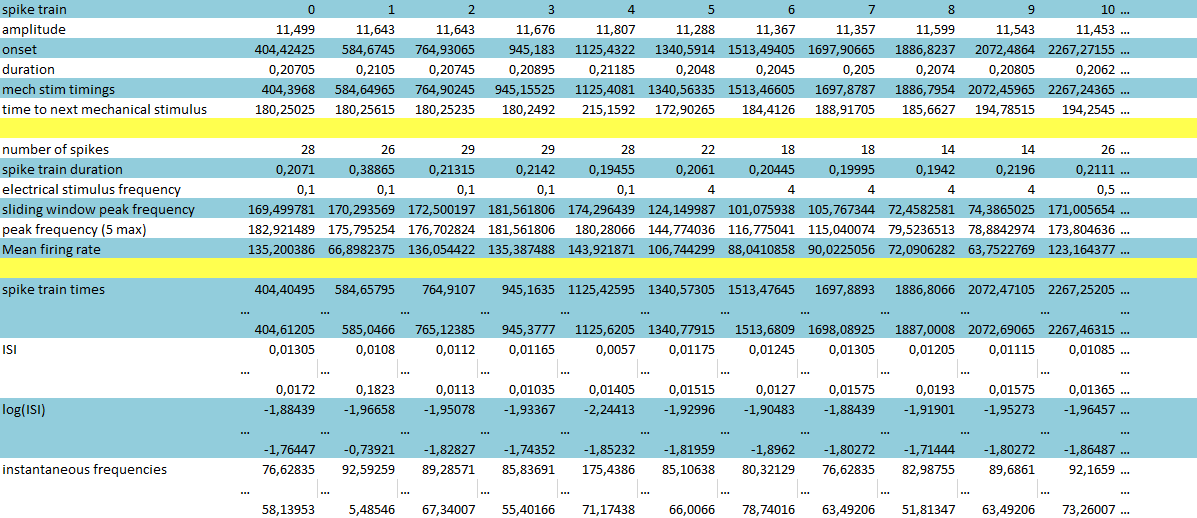
\includegraphics[width = \textwidth]{src/pic/sc_table}
	\caption{Sample picture of table after successful analysis }
	\label{fig:table_sc}
\end{figure}

\subsubsection{Event plot}
A figure that we have seen previously in this thesis is the event plot \ref{fig:eventplot}. It shows an overview of spiking activity after mechanical stimuli over the course of a whole recording. It is not meant to be an in depth analysis tool, but rather a quick visual representation of a recording.

\subsubsection{Comparative diagrams for quantifiers}
Having computed the quantifiers is all well and good, but now we want to visually compare them in order to see if there is correlation between them in any way.
\begin{figure}
	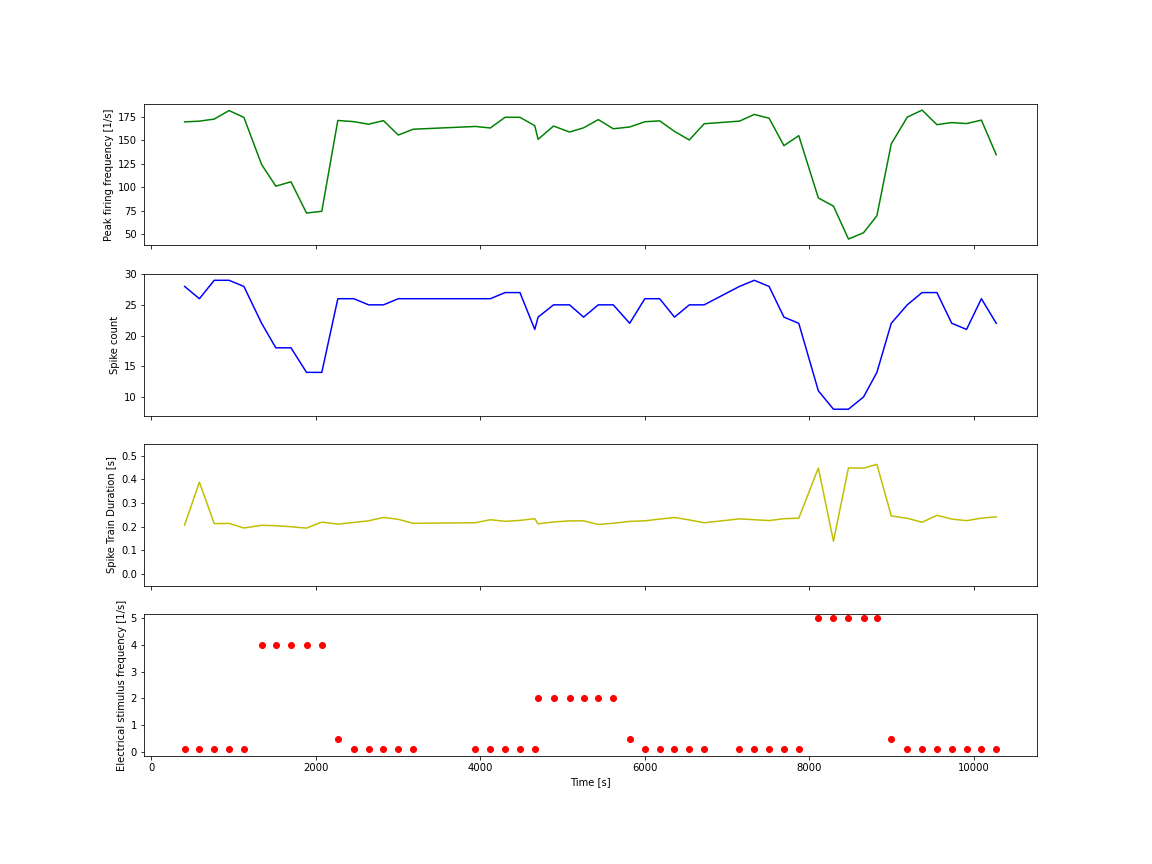
\includegraphics[width = \textwidth]{src/pic/11_12_13_sp}
	\caption{Diagram showing a separated comparison of peak firing frequency and spike count for recording 21}
	\label{fig:quantcomp_sp}
\end{figure}
\begin{figure}
	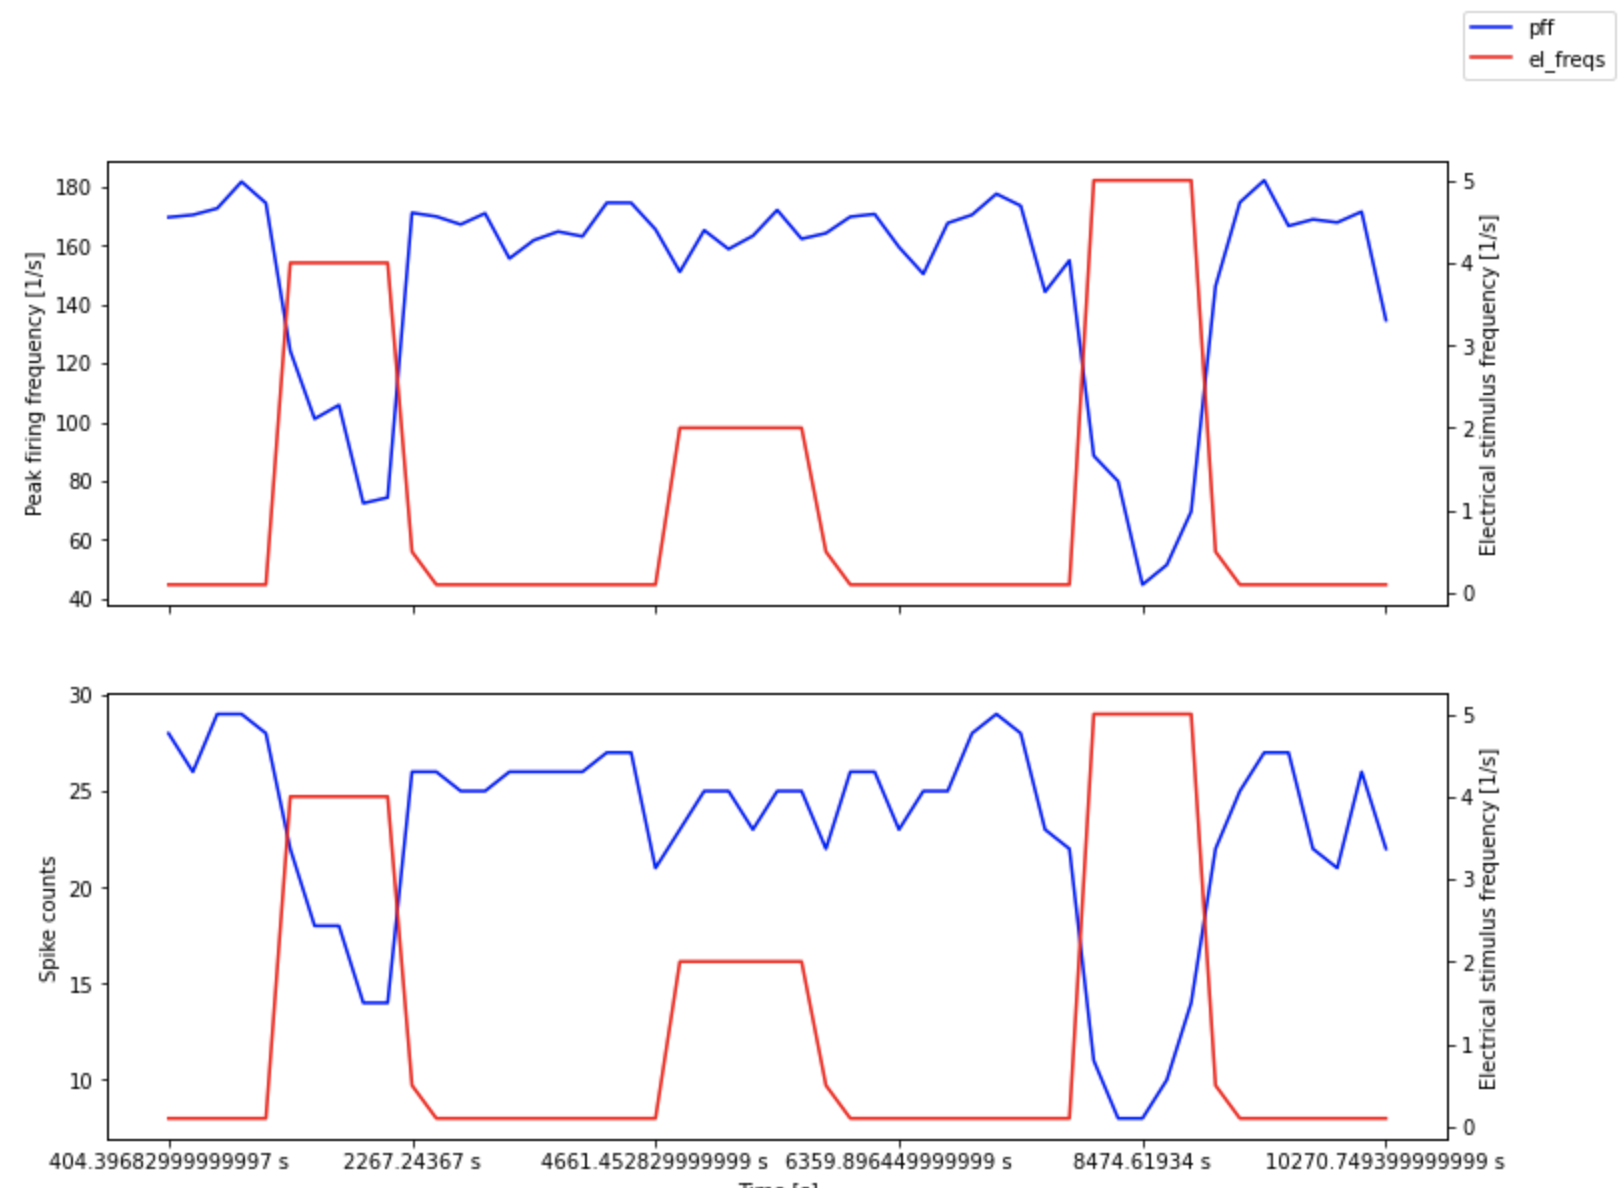
\includegraphics[width = \textwidth]{src/pic/11_12_13_cm}
	\caption{Diagram showing a comparison of peak firing frequency and number of spikes for recording 21}
	\label{fig:quantcomp_cm}
\end{figure}

A good visualization of this can be seen in figures \ref{fig:quantcomp_sp}. This figure compares the spike count with the Peak firing frequency in recording 21. The time is plotted on the x axis ranging from the start of the recording to the end. This recording lasted over 10000 seconds. For each spike train we plotted the Peak firing frequency, the spike count as well as the Spike train duration in separate rows of the figure. In addition we added the electrical stimulation frequency, to see what effect the changes in frequency have on different quantifiers. Figure \ref{fig:quantcomp_cm} shows the same data in a slightly different format. Here the electrical stimulation frequency is included in the rows where we plot the quantifiers to better see the immediate effect.\\
The first thing that we can observe is that the Peak firing frequency and spike count behave very similarly and have almost the exact same graph. Secondly, the application of different electrical stimuli does seem to have an effect on the spike trains. We can see that in the areas with 4 and 5 Hertz stimulation the peak firing frequency as well as the spike count take a significant dip. However, the same cannot be said for the interval with 2 Hertz stimulation. The quantifiers stay largely the same, which leads us to the assumption that there is some sort of threshold which needs to be passed in order to influence the spike trains. In our recordings this threshold seems to lie somewhere between the 2 and 4 Hertz electrical stimulation marks.
While the peak firing frequency and spike count show significant variation, the pike train duration stays pretty constant for the 4 Hertz stimulation but does also increase during 5 Hertz stimulation. This may point to different thresholds for different aspects of a spike train.

\subsubsection{Instantaneous frequencies}
\begin{figure}
	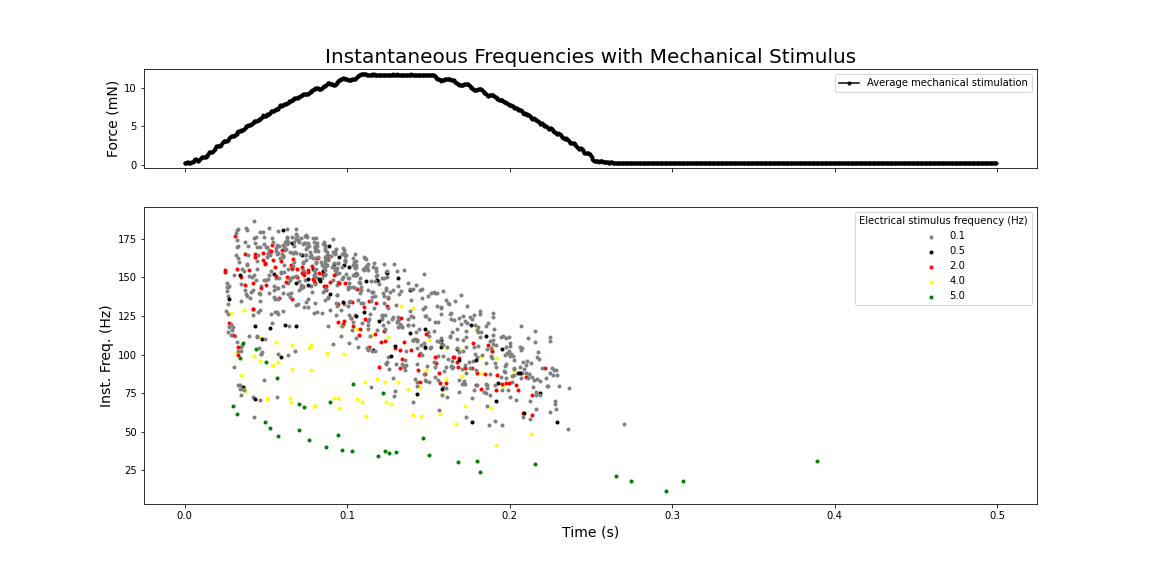
\includegraphics[width = \textwidth]{src/pic/11_12_13U1b_inst_freqs}
	\caption{Figure showing the instantaneous frequencies in each spike train for one recording.}
	\label{fig:inst_freqs}
\end{figure}
Another quantifier that we can take a look at is the instantaneous frequencies of the spikes in the spike trains and observe how these change with different levels of electrical stimulation. To visualize this we recreated a figure from the original paper from Roberto de Col in Figure \ref{fig:inst_freqs}. The data for this figure is taken from recording 21. The x axis depicts the time since the last stimulus in seconds. The top part of the figure shows the force of mechanical stimulation that evoke the spike trains. This curve represents the average mechanical stimulus in this recording. A sliding window of three was used for the calculation of the instantaneous frequencies to smooth out some of the outliers. The lower part of the figure is a scatterplot of these instantaneous frequencies for every spike train in the recording. They were color-coded according to the underlying electrical stimulation frequency. The pike trains with the base level frequency of 0.1 Hertz are colored in gray, while the trains with higher stimulation are colored in red, orange and yellow for an electrical frequency of 2, 4 and 5 Hertz respectively. Finally the trains with a stimulation of 0.5 Hertz stimulation frequency are colored in blue. From the scattering of the dots we can observe that the spike trains occurring during an electrical stimulation of 4 and 5 Hertz show lower instantaneous frequencies than the base level spike trains. The red dots lie mostly in the main cluster of dots belonging to the base level spike trains, which would fit with the previous figures and the assumption of some sort of threshold for spike train alterations.



%selected additional information in more detail:

%-diagram of peak firing frequency, spike counts, train duration and electrical frequency\\
%-shows the correlation between electrical frequency and the other quantifiers of single spike trains\\

%-diagrams of Interspike Intervals(isi) and logarithm of isi\\
%-should show that by taking the logarithm, the isi becomes more linear\\




\cleardoublepage


%\chapter{Software}

-Use-cases:\\
	\null\quad-opening data (importing)\\
	\null\quad-latency study (Alina)\\
	\null\quad-chemical data study (Jessica)\\
	\null\quad-mechanically evoked spike trains (Alexander)\\
	\null\quad-experimental researchers (Barbara)\\
-results in a list of requirements\\
-Use-cases lead to software engineering approach\\
-nessecary steps for my analysis\\
-how I implemented it



\begin{comment}
Alina \\
Works with spike2 data \\
Electrical data and mechanical data \\
Uses old way of importing currently (csv export from spike2) \\
Needed channels from csv export: \\
DigMark for electrical and mechanical stimulus events \\
WaveMark channel for timestamps of spikes \\
Information used: \\
Electrical stimulus events + timestamps \\
Calculate Latency for spikes (timestamps) \\
Calculate Spike Count  \\
In theory this information is available with the direct import of openMNGlab right now \\
Potential problems with direct openMNGlab importer: \\
Each template for spikes in spike2 results in separate channel in Neo structure after openMNGlab import -> needs some filtering (manual right now) \\
Electrical and mechanical events share a channel (DigMark) and somehow need to be distinguished if the recording also features mechanical stimulation \\
\end{comment}

The first user is a student who does data analysis on mechanically and electrically stimulated Spike2 data. The goal is to perform latency analysis for spikes.  The raw spike2 files feature a lot of information, not all of which is always needed. In this case, all that is required to analyse the latencies of the spikes are the timestamps of the spikes itself and the timestamps of the stimulation events. For the Spike2 software this means that we need to extract the DigMark channel which contains the event information as well as the wavemark channel which contains the information on the already presorted spikes.\\
The relevant information can be imported using the importing function of openMNGlab. 
 
\begin{comment}
Alexander \\
Works with spike2 data \\
Electrical and mechanically stimulated data \\
Uses a mixture of old and new importing currently \\
Needed channels from csv export: \\
Mechanical force channel \\
Spike channel for timestamps of spikes \\
Need channels from direct spike2 import: \\
Electrical stimulus channel \\
Information used: \\
Electrical stimulus events + timestamps \\
Mechanical stimulus events (duration, amplitude) + timestamps \\
Timestamps for spikes in spike trains \\
Potential problems with the Neo importer: \\
Each template for spikes results in separate spike channels in the Neo structure -> this means that the filtered spikes in the spike2 spike channels (e.g., nw-1…) need to be bundled together again \\
Mechanical force channel import does not work currently \\
Electrical and mechanical events share a channel (DigMark) and somehow need to be distinguished \\
After the import of the mechanical force channel, the mechanical stimuli need to be filtered as such (probably will not happen automatically by the importer) \\
\end{comment}

The second user is also a student who uses mechanically and electrically stimulated Spike2 data. His goal is to analyse spike trains resulting from mechanical stimulation. For this he needs also does not need all of the information contained in the raw Spike2 file. He needs the event information for mechanical and electrical stimuli as well as the mechanical force information for details of the mechanical stimuli. As well as the first user he also needs the information collected from the wavemark channels detailing the exact spiking patterns.

\begin{comment}
Jessica \\
Works with spike2 data \\
Chemical data \\
Uses Neo importer \\
Needed channels from import: \\
Spike channels for spike timestamps \\
Information used: \\
Intervals which are relevant for the application of chemicals \\
Spikes + timestamps inside those intervals \\
Which chemicals are applied when \\
Potential problems with openMNGlab importer: \\
The chemical protocols are not automatically importable and readable; There is a channel in spike2 for comments where this information is given in theory, however, the notation of what is given and how much varies from comment to comment, and one needs a good understanding of the chemicals and potentially experimental procedure \\
Comments channel is not being imported currently, even if the chemical notes where uniform; This means one must manually reed the comment channel in the spike2 software itself and manually choose some intervals which might be promising for observing chemically induced changes in spiking activity \\
\end{comment}
 

Which information should available after importing data? \\
Spikes + timestamps \\
Electrical stimulation + timestamps \\
Mechanical stimulation + timestamps, duration, amplitude \\
Information about application of other stimuli (chemicals, heat…) \\
For human data: temperature?  

Spike2 \\
Spike channels + some way to group them easily (e.g., in groups from spike2 templates) \\
Electrical event channel + some way to distinguish between electrical and mechanical events \\
Mechanical force channel (maybe optional) \\
Comments channel (maybe optional) \\
Temperature (optional) (probably needed for human data) \\

\begin{comment}
My steps in analysis: 

First, I used a jupyter notebook from Radomir. For this the data needed to be extracted from Spike2 directly in the Software. This export step leads to a single csv file for one recording with 5 channels: Time, Signal, Force, DigMark(stimulation events), Spikes 

Using the csv files I could extract the spike trains for each mechanical stimulation. The detection of the spike train worked as follows: The start of the spike train gets determined by the stimulation event. The length of the spike train is a previously set amount of time (in most cases 500ms). During this timeframe all spikes in the spike channel get put into a list that keeps track of the spike trains. This pretty basic detection of spike trains works well in this specific use case but has its limits when it comes to other kinds of data with other experimental protocols or just simply recordings without any protocols. Then because we do not have the exact starting points of the trains or bursting patterns this method of detection falls flat. 

This first jupyter notebook already made use of what later became openMNGlab. The import of the data was handled by the software framework. However, openMNGlab got some updates soon after which made some significant changes to how the importers work. In the new and improved framework, the importer worked on the original Spike2 files instead of the extracted csv files. This allows for more detailed representation of the data since much of the information was lost in the extraction before this update. However, with this new way of importing the data the mechanical stimulation was not able to be extracted. I still needed the information of the mechanical stimulation which was only contained in the extracted csv file. For this reason, in my analysis from here on, I used a hybrid of the old and new versions of openMNGlab until I was able to fix the new importer to also include the mechanical stimulation channel. 
\end{comment}

\cleardoublepage


%\chapter{Analysis}

In this chapter I will present the results of my analysis.\\
-I will present the results with the help of diagrams\\

-Describe the analysis that is done for each recording file we have:\\
-Show picture of a table with all the quantifiers as an axample and add the rest to the appendix\\
\begin{figure}
	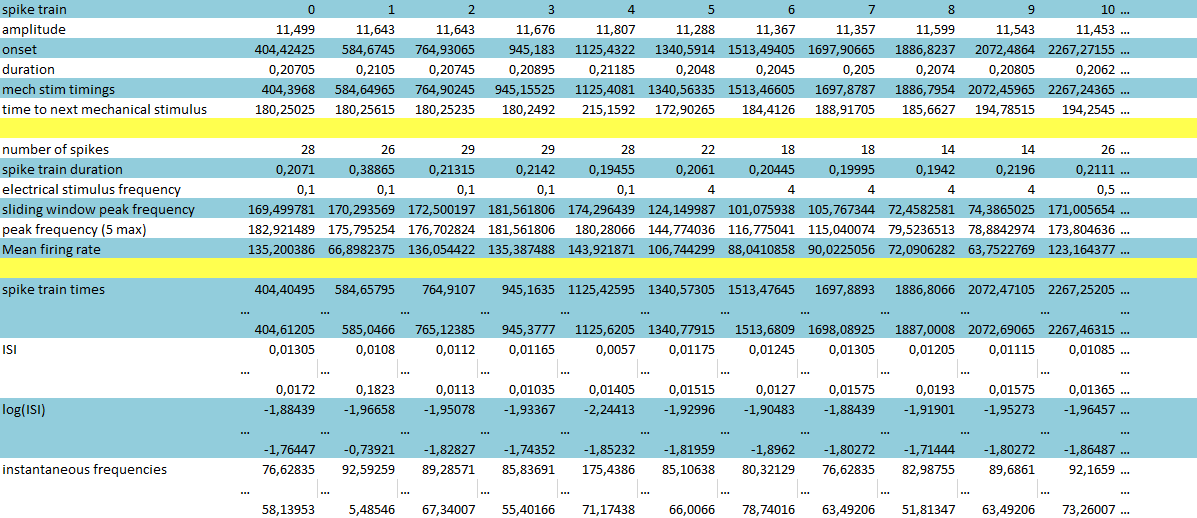
\includegraphics[width = \textwidth]{src/pic/sc_table}
	\caption{Sample picture of table after successful analysis }
	\label{fig:table_sc}
\end{figure}
-first batch contains information on the mechanical stimulus, second batch single number quantifiers about spike train, last batch lists of raw data and list quantifiers such as ISI\\
-with the help of this diagram describe the quantifiers and results that were computed\\


ausgewähltes in more detail:

-diagram of peak firing frequency, spike counts, train duration and electrical frequency\\
-shows the correlation between electrical frequency and the other quantifiers of single spike trains\\

-diagrams of Interspike Intervals(isi) and logarithm of isi\\
-should show that by taking the logarithm, the isi becomes more linear\\




\cleardoublepage


\chapter{Discussion}
\begin{comment}
-speak about the problems with the software
- what needs to be fixed


-analysis:
-threshold, already mentioned in Robertos paper
-active nerve fiber has decreased response
-not linear

hdf5 not yet feasible, since we get 3 separate data structures and not one single concise format.


In this chapter I will discuss the results presented in the previous chapter and think about possible future work regarding the analysis. Also I will discuss the integration of my code (quantifiers mainly) into openMNGlab and thoughts about the structuring of the software.
\end{comment}
\section{Software}
This thesis included working with multiple versions of the openMNGlab framework. The biggest issue with the software at this point are the importing capabilities. This is a very crucial functionality necessary for everyone who works with the software. Different users have reported that not all aspects are imported into the framework, such as the "Comments" channel containing the experimental protocol in chemical recordings. 

There are other cases where the functionality can be improved. In this thesis, there were difficulties importing everything that was needed for the analysis. With the current Neo importer and mechanically and electrically stimulated data, there is mechanical information that gets lost, when just using the current framework version. This is something that has to be rectified and the import of the mechanical force channel, as well as the missing wavemark channels might be possible in the future. 

Another topic worth discussing, is the possibility of storing the data and having the option of reloading it at a later time. This would lead to faster loading times, when revisiting already analyzed data. Neo supports this by providing the option to save Neo objects to the hdf5 file format. This could be used for the thesis data only if everything can be imported by the Neo importer and put into one single data structure, which is another reason to look into this in the future. 

Since every experiment produces different data with different specifications, there might come a point in the future, where new issues with new data sets arise.

\section{Spike Analysis}
In Chapter~\ref{results_chapter}, we have seen what effect continuous nerve fiber activity can have on the response to a new stimulus. With increased fiber activity, induced by electrical stimulation, the spike train elicited by a mechanical stimulus changed in comparison to the control. The higher the electrical stimulation frequency gets, and with it the fiber activity, the fewer spikes are produced by the mechanical stimulus. This relation is not linear, however. There seems to be a threshold of electrical stimulation frequency after which we notice a change in response to the mechanical stimuli. In Figures~\ref{fig:quantcomp_sp},~\ref{fig:inst_freqs} we see that an electrical background stimulation frequency of up to 2 Hz does not seem to have any effect on the peak firing frequency or the number of spikes per train. With the 4 and 5 Hz stimulation, however, we see a noticeable dip in peak firing frequency and number of spikes per train. This would suggest that a high load on the nerve fiber hinders the regular response to the mechanical stimulus that we see without much activity on the nerve fiber. This corresponds well with the results found by Uebner et al.~\cite{roberto}.

In this thesis, the detection of spike trains is very basic. We get the start time by the event marker in the recording file and then define the spike train as all the spikes that appear in a period of up to 500 ms after that event. For the purposes of these experiments this is enough, since we will always know when the spike trains are supposed to happen. When this sort of analysis gets expanded to also search for randomly appearing spike trains in patients in the future, there needs to be more sophisticated ways to detect spike trains when there is no way to know exactly when one will happen.

Another interesting aspect for the future is the integration of Elephant into the existing analysis. Since Elephant is also a Python module and implements advanced analysis functions for spike trains it might serve as a good addition. 

In this thesis, we focused mostly on the analysis of single recordings from mechanically and electrically stimulated rats. This could be expanded to more big picture statistics comparing multiple different recordings in a broader context than in this thesis, as well as comparing differing stimulation types. These statistics could give a better understanding of nerve fiber responses as a whole.





\cleardoublepage


%\chapter{Code Listings}\label{ch:listings}
%% use language 'myLng' for the next listings (until another language is set)
%% include listing 'listings/AdverseReactionApp.aj' with label and caption
%% note: big listings sometimes need to overwrite the float value that has been
%% already set in the general listings setup (see paper.tex)

This chapter contains the beautiful listing \ref{lst:system}. 
Lorem ipsum dolor sit amet, consetetur sadipscing elitr, sed diam nonumy 
eirmod tempor invidunt ut labore et dolore magna aliquyam erat, sed diam 
voluptua. At vero eos et accusam et justo duo dolores et ea rebum. Stet 
clita kasd gubergren, no sea takimata sanctus est Lorem ipsum dolor sit 
amet. Lorem ipsum dolor sit amet, consetetur sadipscing elitr, sed diam 
nonumy eirmod tempor invidunt ut labore et dolore magna aliquyam erat, 
sed diam voluptua. At vero eos et accusam et justo duo dolores et ea 
rebum. Stet clita kasd gubergren, no sea takimata sanctus est Lorem 
ipsum dolor sit amet. 




\begin{figure}[hbt]
\lstset{language=MontiArc}
\lstinputlisting[
label=lst:system,
caption=Code listing with user defined syntax highlighting (MontiArc).] {src/listings/AdverseReactionApp.aj}
\end{figure}

\cleardoublepage


\chapter{Conclusion}
In this thesis spike train analysis in mechanically and electrically stimulated rat neural fibers was studied. This analysis was tested as a use case for the openMNGlab software. As a proxy for human MNG data single nerve fiber recordings from the skin nerve preparation of rats was used. The fiber was electrically stimulated to evoke different levels of spike activity, to study the effect of previous nerve fiber activity on the response to mechanical stimuli. 
The result of this was that the more the nerve fiber was active, the less was the response to mechanical stimuli. After a threshold of 2 Hz of electrical stimulation frequency the mechanically evoked spike trains contain noticeably less spikes and the peak firing frequency is significantly lower.

The openMNGlab framework was used to facilitate the analysis. The analysis of this type of mechanically stimulated data showed that the importing capabilities of the software needs improvements. Not all of the data could be loaded with the standard tools included in the framework. Other users also reported issues with the importers of openMNGlab, which is where the main work in the near future lies. The code used in this bachelor thesis can be found under \url{https://github.com/alexandertartsch/Bachelor_thesis_code/tree/v1}

% Bild einbinden
%\begin{figure}[ht!]
%\begin{center}
\includegraphics[width=5cm]{src/pic/logo}\end{center}
%\caption{Das SE Logo}
%\label{Logo}
%\end{figure}

\cleardoublepage


\bibliographystyle{alpha}
\addcontentsline{toc}{chapter}{References}
\bibliography{src/bib/references}

% Begin Anhang
\appendix
\chapter{z.\,B. Programmdokumentation}

\cleardoublepage


\end{document}
